\subsection{Application to the test vehicle}
\label{sec:application-test-vehicle}

The method described in both previous sections (\ref{sec:block-failure-cz} and \ref{sec:block-chaining}) is tested in simulation on the regulation function of the testchip.
The testchip was presented in section \ref{sec:supply-desc}, and it was shown that negative rectangular pulses can generate functional failures in it.
The regulation function is composed mostly of a pre-regulator, a bandgap and a regulator.

One input and one output per block were selected (Table \ref{selected-pins-for-cz}) for validating the characterization method.
V\textsubscript{batt} is the input pin of the pre-regulator and is also exposed externally.
It is the battery input connection and constitutes a very likely \gls{esd} entry point.
Nominal voltage on this pin is expected near \SI{14}{\volt}.

V\textsubscript{clamp9} is a \SI{9}{\volt} output supply from the pre-regulator and an input for the bandgap.
The bandgap block cannot operate without this supply voltage.
This is why this pin was selected for the characterization.
The failure criteria is set at \SI{0}{\volt}, corresponding to a level where the ESD causes V\textsubscript{clamp9} to go negative, which is a worse situation than without any DC supply.

V\textsubscript{ref1p0} is the \SI{1}{\volt} bandgap output reference.
It is the main signal required by the regulator to produce the final \SI{2.5}{\volt} V\textsubscript{2p5} regulated supply.
Failure criteria of V\textsubscript{ref1p0} is chosen at \SI{0.5}{\volt}, half the operating voltage.
The choice of this particular level is not strict and another value could have been chosen.

V\textsubscript{2p5} is the output of the regulator and the last signal in the considered function.
It is an external node, that requires a large \SI{100}{\nano\farad} decoupling capacitance.
This output is used further in the original circuit to supply digital cells.
The failure criteria for this net is chosen at \SI{2.1}{\volt}.
Below this value, digital cells are no longer guaranteed to operate properly.

\begin{table}[!h]
\centering
\begin{tabular}{@{}llll|ll@{}}
\toprule
input pin  & DC value (V)    & stress amplitude           & stress width                                    & output  & fail criteria \\ \midrule
vbatt      & \SI{14}{\volt}  & \SIrange{-1}{-10}{\volt}   & \SI{1}{\nano\second} to \SI{1}{\micro\second}   & vclamp9 & < \SI{0}{\volt}       \\
vclamp9    & \SI{9}{\volt}   & \SIrange{-1}{-15}{\volt}   & \SI{10}{\nano\second} to \SI{10}{\micro\second} & vref1p0 & < \SI{0.5}{\volt}         \\
vref1p0    & \SI{1.0}{\volt} & \SIrange{-0.5}{-10}{\volt} & \SI{10}{\nano\second} to \SI{10}{\micro\second} & v2p5    & < \SI{2.1}{\volt}      \\
\bottomrule
\end{tabular}
\caption{Selected pins for characterization and characterization limits}
\label{selected-pins-for-cz}
\end{table}

\subsubsection{Per-block characterization}

% Talk about the characterization limits
The characterization is done using negative voltages, to reproduce failures observed previously with the testchip.
It was observed for a sufficiently high negative voltage that a short pulse can cause a full restart of the primary supply and the V\textsubscript{2p5} signal.
The time taken by this restart is several order of magnitudes longer than the original pulse injected on the pre-regulator input.

% Which load value for characterization
The characterization setup for each block is provided in Fig. \ref{fig:block_function_cz_regu}.
They require a characterization load to simulate the impact of neighbor blocks, initially modeled with a \SI{1}{\mega\ohm} resistor.
A high-impedance avoids drawing too much current on the output, which could affect or prevent normal operation.
This value is not chosen in a strict manner and other values could have been chosen.
The goal is to perform a preliminary test.
The impact of this load on the characterization is evaluated later on in the analysis.

%
The regulator setup (characterization C) is more complex because the characterized input is not a supply but a \SI{1.0}{\volt} reference.
The regulator must also be powered, and a \SI{9}{\volt} DC supply is added for this purpose.
A \SI{100}{\nano\farad} decoupling capacitor is also connected on the output because it is required by the regulation function.
The regulator needs a low-power biasing signal called V\textsubscript{clamp2p5}, that is normally generated by the bandgap in the real circuit.
This connection is represented in orange in the Fig. \ref{fig:block_function_cz_regu}.
In the setup provided here, blocks are characterized independently in different testbenches, therefore the bandgap and regulator cannot be connected together.
Therefore, the orange connection cannot be made between the two blocks.
V\textsubscript{clamp2p5} is left floating on the bandgap output.
For the regulator, the biasing signal is modeled with a \SI{2.5}{\volt} DC supply in series with a \SI{1}{\kilo\ohm} resistor.
The impact of the removal of this connection on the failure signature is discussed later in section \ref{sec:impact-missing-conns}.

\begin{figure}[!h]
  \centering
  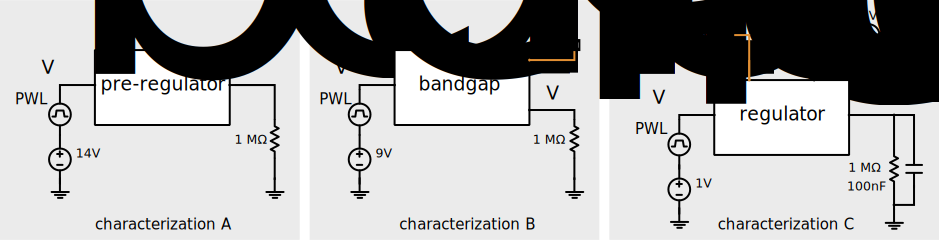
\includegraphics[width=\textwidth]{src/4/figures/characterization_setup_regu.pdf}
  \caption{Block characterization setups}
  \label{fig:block_function_cz_regu}
\end{figure}

% Simulation process
A set of simulations is run with those characterization setups.
The only varying parameters are the input pulse amplitude and input width of each PWL source.
Ranges for these parameters were given previously (Table \ref{selected-pins-for-cz}).
This type of parameterized simulations can be efficiently distributed on multiple machines.
Characterization results are provided in Figs. \ref{pre_regu_wb}, \ref{bandgap_wb} and \ref{regu_wb}.

\begin{figure}[!h]
  \centering
  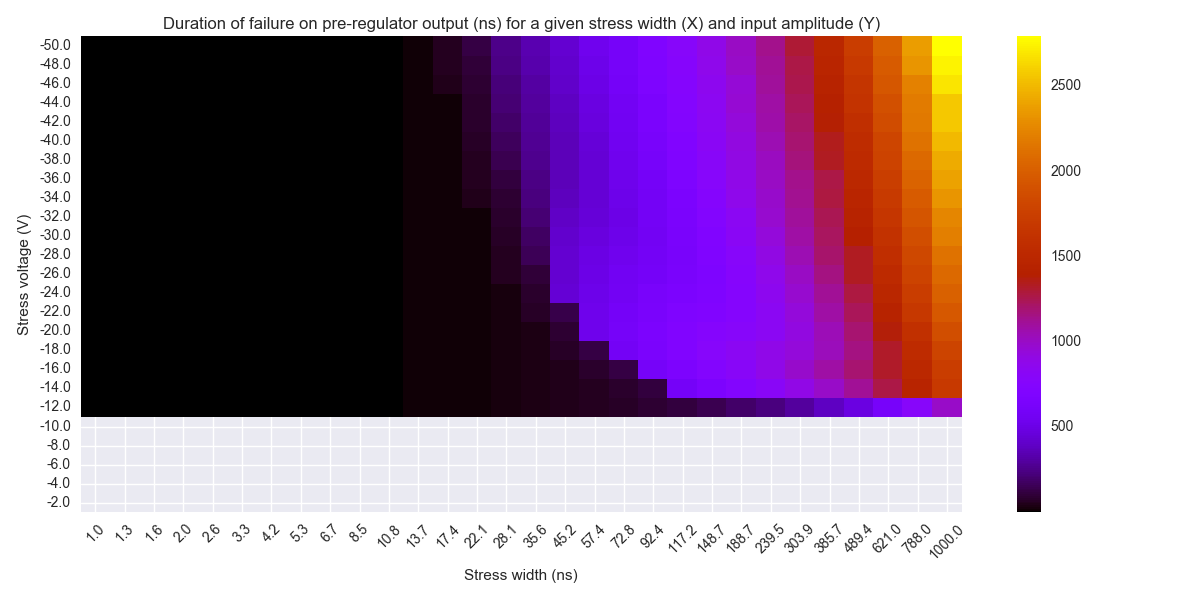
\includegraphics[width=\textwidth]{src/4/figures/preregulator_cz.pdf}
  \caption{Pre-regulator V\textsubscript{clamp9} failure matrix}
  \label{pre_regu_wb}
\end{figure}

\begin{figure}[!h]
  \centering
  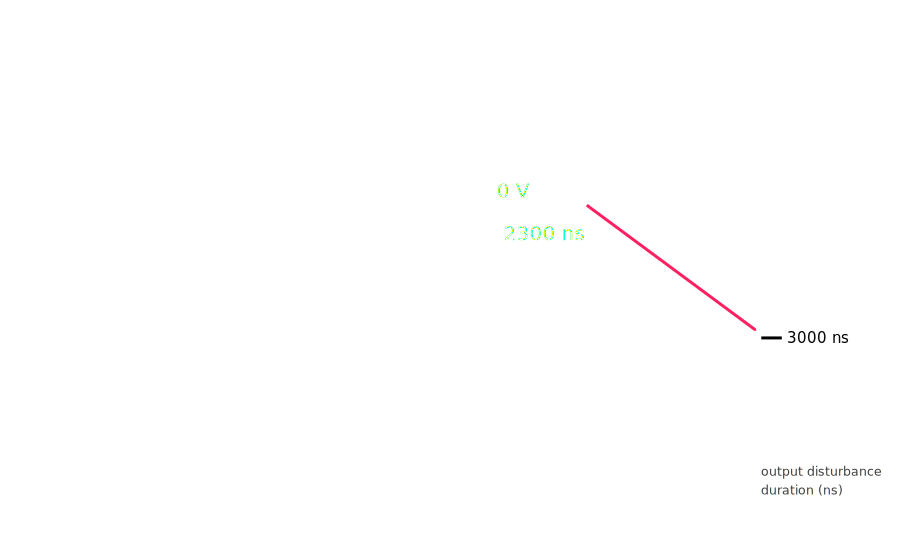
\includegraphics[width=\textwidth]{src/4/figures/bandgap_cz.pdf}
  \caption{Bandgap V\textsubscript{ref1p0} failure matrix}
  \label{bandgap_wb}
\end{figure}

\begin{figure}[!h]
  \centering
  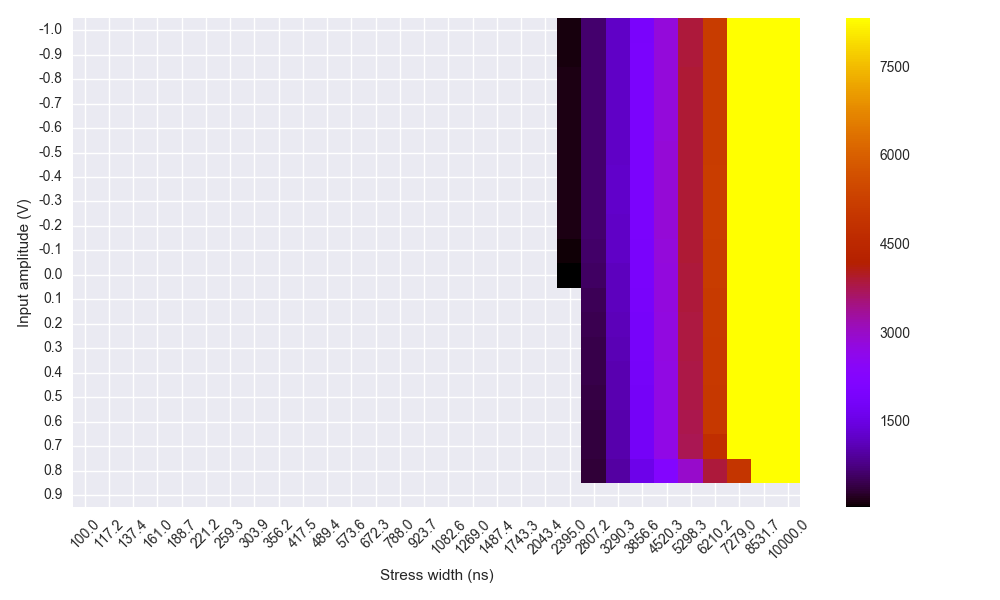
\includegraphics[width=\textwidth]{src/4/figures/regulator_cz.pdf}
  \caption{Regulator V\textsubscript{2p5} failure matrix}
  \label{regu_wb}
\end{figure}

\subsubsection{Model chaining}

% Characterization done, now perform chaining
After the characterization phase, it is now possible to chain the models together.
The goal is to evaluate the entire function's robustness.
A rectangular pulse is injected on the global input (pre-regulator input).
The chain of models is employed for predicting without running any simulation whether or not a failure will be found on the output pin.
The input stress is generated by a \gls{tlp} generator, producing a pulse of \SI{1}{\micro\second} duration with a \SI{-30}{\volt} amplitude.

% Do it on one pulse config
Therefore, coordinates (\SI{1}{\micro\second}, \SI{-30}{\volt}) are reported on the pre-regulator failure matrix (Fig. \ref{pre_regu_wb}).
This point indicates a failure on V\textsubscript{clamp9} below \SI{0}{\volt} (failure criteria) for a duration of \SI{2300}{\nano\second}.
Coordinates (\SI{2300}{\nano\second}, \SI{0}{\volt}) are reported on the bandgap's failure matrix (Fig. \ref{bandgap_wb}).
This point indicates a failure on V\textsubscript{ref1p0} below \SI{0.5}{\volt} for a duration of \SI{3000}{\nano\second}.
Coordinates (\SI{3000}{\nano\second}, \SI{0.5}{\volt}) are reported on the regulator's failure matrix (Fig. \ref{regu_wb}).
With those coordinates, the final signal V\textsubscript{2p5} is estimated to fail (< \SI{1.25}{\volt}) during \SI{1500}{\nano\second}.

% Summarize results
The model chain estimates that the regulation function will fail during \SI{1500}{\nano\second} for a \SI{-30}{\volt} \SI{100}{\nano\second} stress on the input.

% Perform standard complete simulation for reference
This result is tested against a simulation of the regulation function.
The simulation setup is given Fig. \ref{fig:reference_simu_circuit}.
This simulation uses the full block schematic but the blocks are connected together only through the nets V\textsubscript{clamp9} and V\textsubscript{ref1p0}.
For instance, the biasing signal in orange is still kept disconnected between the two blocks.
This simulation serves as a reference for evaluating the model chain.

\begin{figure}[!h]
  \centering
  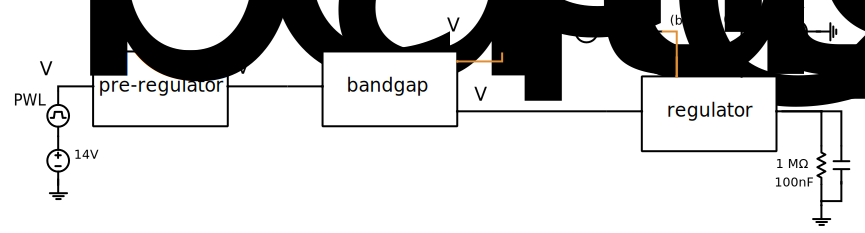
\includegraphics[width=\textwidth]{src/4/figures/characterization_setup_regu_complete.pdf}
  \caption{Reference simulation circuit}
  \label{fig:reference_simu_circuit}
\end{figure}

% What is injected
The complete simulation is ran with the same \SI{-30}{\volt} \SI{1}{\micro\second} input stress than the model chain.
Signals V\textsubscript{batt}, V\textsubscript{clamp9}, V\textsubscript{ref1p0} and V\textsubscript{2p5} are compared with values obtained from the model chain.
Simulation results are provided in Fig. \ref{fig:reference_simu}.
The model chain results are also plotted on the curve (red waveforms).
Those waveforms are simply generated with the duration and amplitude predicted by the model chain.

\begin{figure}[!h]
  \centering
  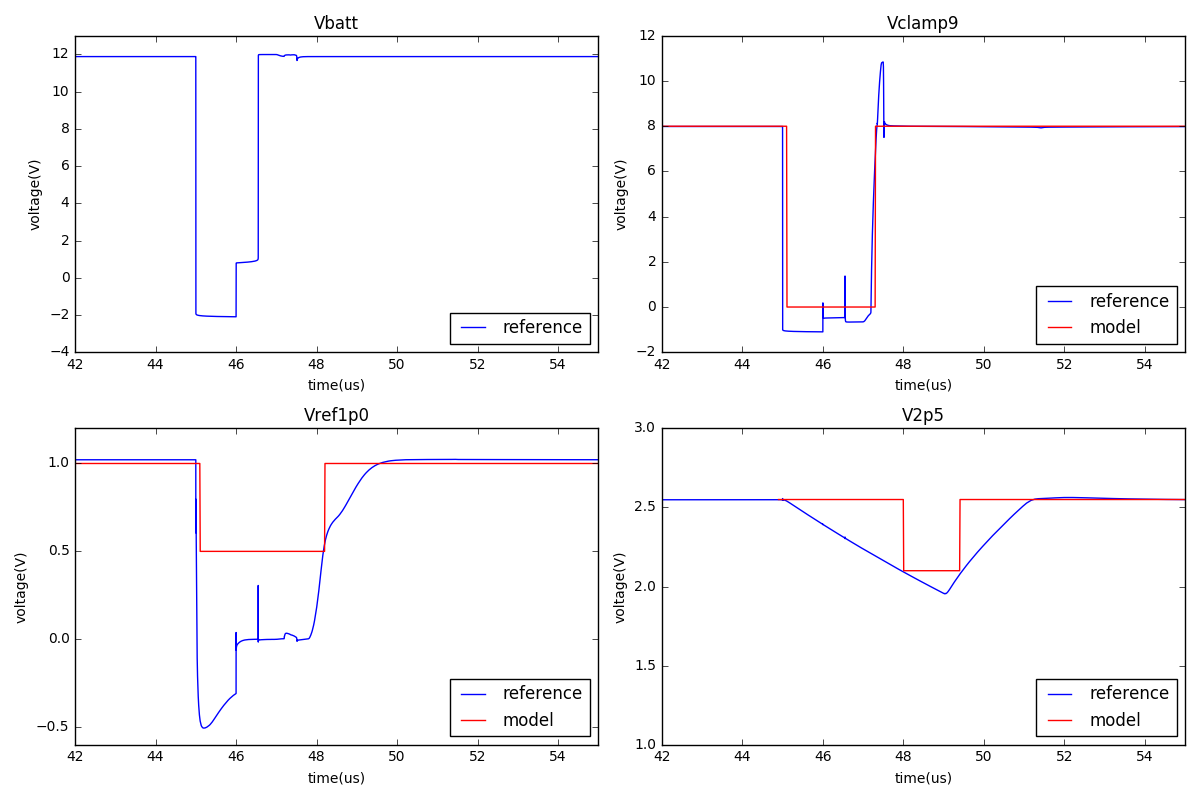
\includegraphics[width=\textwidth]{src/4/figures/total_simulation_30V_1u.png}
  \caption{Reference simulation waveform - TLP stress \SI{-30}{\volt} \SI{1}{\micro\second}}
  \label{fig:reference_simu}
\end{figure}

% Comment the results
Overall, the model chain predicts quite well the disturbance on the output of each block.
V\textsubscript{batt} has no waveform model because it is the input external signal.

% Vclamp9
V\textsubscript{clamp9} is well modeled and both waveforms match quite well.
It should be noted that the correlation on the amplitude between model and simulation is purely incidental.
It is due to the fact that the failure criteria was arbitrarily set at \SI{0}{\volt}, and that the block circuit design tends to clamp the output voltage near \SI{0}{\volt} in case of a negative disturbance.

% Vref1p0
The width of V\textsubscript{ref1p0} is also correctly modeled and matches the reference.
On the other hand, the amplitude shows a large correlation difference.
Here again, the design seems to clamp the output voltage near \SI{0}{\volt} on negative transients.
Since the failure criteria is set above that at \SI{0.5}{\volt}, both curves do not match.

% V2p5
Large differences are observed for V\textsubscript{2p5} between model and reference.
They are due to the triangular shape of the signal, that cannot be properly modeled with the rectangular shape.
It is one of the first limitations of the model.
Other limitations are discussed in the next section.
Despite this, the disturbance was detected by the model which is already a good achievement.

% Transition with next section
This first simulation proved that the model chain method definitely has some potential.
It has also highlighted some limitations.
The next section discusses further pitfalls of the model chain and an improvement is proposed and tested.
